%! Author = joeda
%! Date = 2022-12-19

% Preamble
\documentclass[11pt]{article}

% Packages
\usepackage{amsmath}
\usepackage{graphicx}
\usepackage{caption}
\usepackage{subcaption}

%\usepackage{biblatex}
\usepackage[backend=bibtex]{biblatex}

\usepackage{blindtext}%section management
\usepackage{xcolor} %color management

\newcommand\myworries[1]{\textcolor{red}{#1}}

\usepackage[utf8]{inputenc} % Pour les accents
\usepackage[english]{babel}  % Language hyphenation and typographical rules
\usepackage{csquotes}
% Document
\begin{document}

\section{Data Analysis}

    The first step of any ML project is to analyse the data available to us. We will already split our data between
    training and validation just to simplify our analysis here.

    First, our private data from CIUSSS. We will first look at the distribution of the classes. As we can see in
\ref{fig:hist_ciusss}, the classes are not balanced. We will need to take this into account when training our model.


While we tried to provide a minimum of examples for each class in the validation dataset, we still observe a class imbalance.
We will therefore need to be careful not only to rely on a basic loss for things like a hyperparameter search if we want to
have the best model in more than the over-represented categories. We could, for example, ponder the loss with different weights
by classes

\addbibresource{reference.bib}

\begin{figure}
     \centering
     \begin{subfigure}[b]{\textwidth}
         \centering
         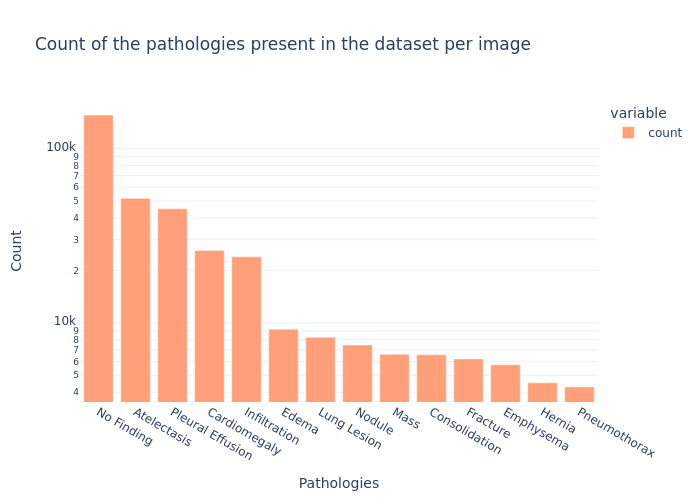
\includegraphics[width=\textwidth]{plots/histogram_ciusss_train}
         \caption{Training}

     \end{subfigure}
     \hfill
     \begin{subfigure}[b]{\textwidth}
         \centering
         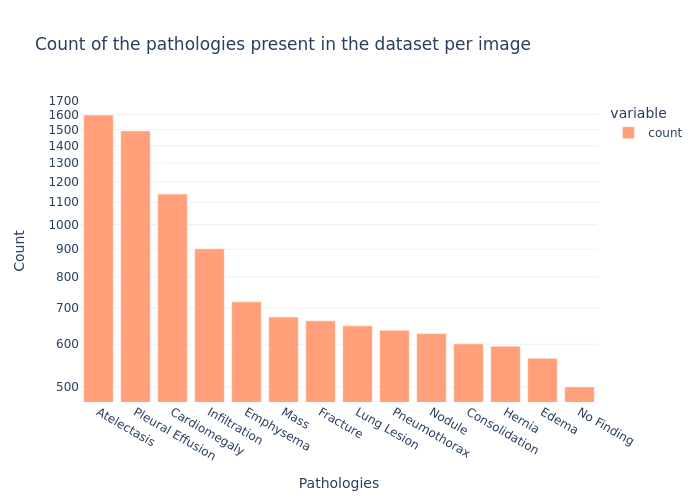
\includegraphics[width=\textwidth]{plots/histogram_ciusss_valid}
         \caption{Validation}

     \end{subfigure}
     \hfill
     \caption{Histogram for the different labels present in the CIUSSS dataset}

     \label{fig:hist_ciusss}
\end{figure}

    Another important thing to look at could be the correlation between diseases, to identify potential biases in the data.

\begin{figure}
     \centering
     \begin{subfigure}[b]{\textwidth}
         \centering
         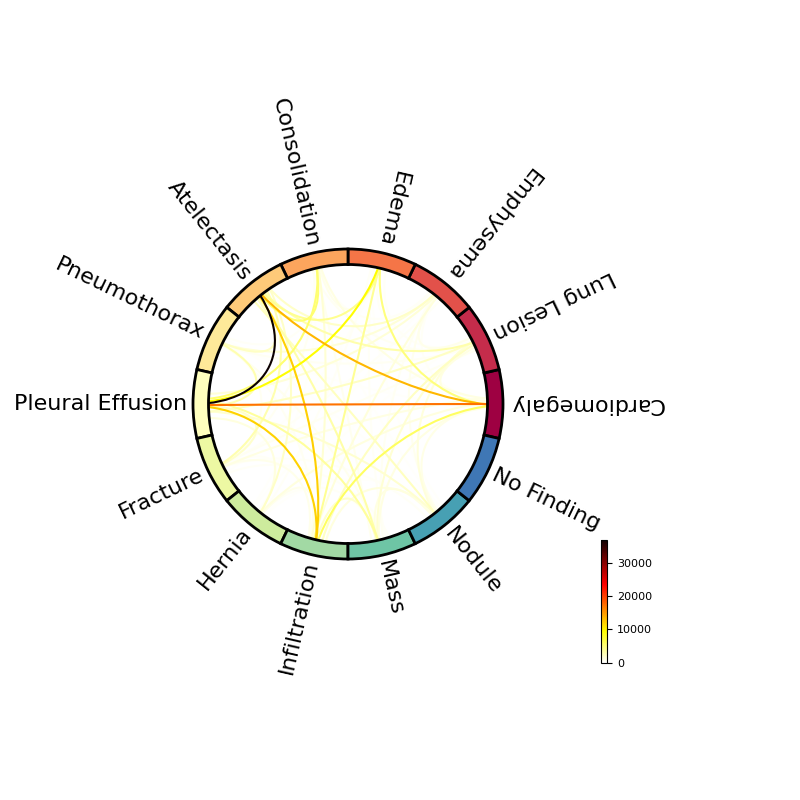
\includegraphics[width=0.75\textwidth]{plots/chords_ciusss_train.png}
         \caption{Training}
         \label{fig:y equals x}
     \end{subfigure}
     \hfill
     \begin{subfigure}[b]{\textwidth}
         \centering
         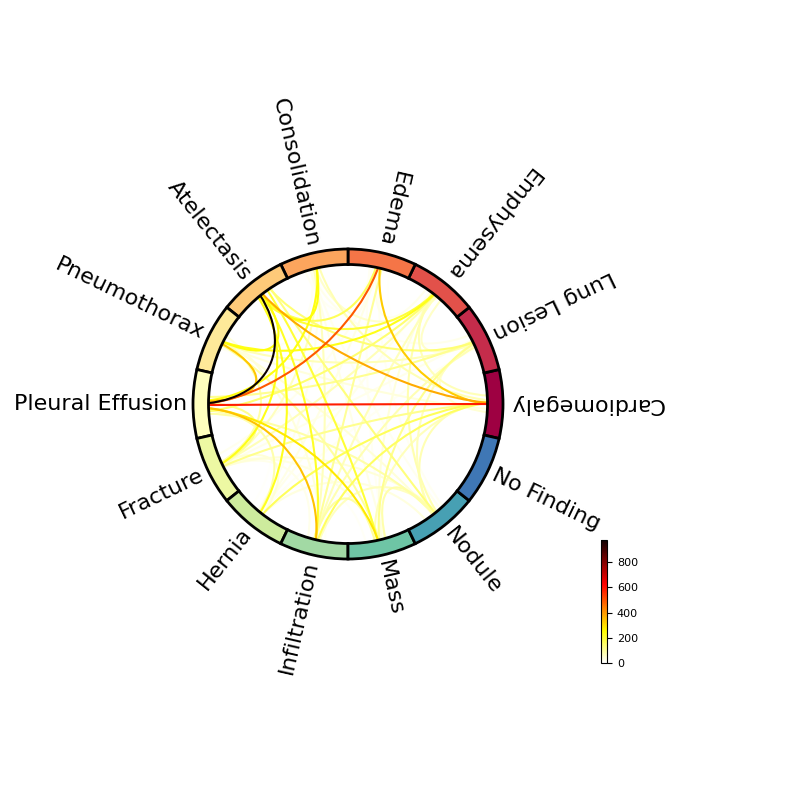
\includegraphics[width=0.75\textwidth]{plots/chords_ciusss_valid.png}
         \caption{Validation}
         \label{fig:correlation_ciusss}
     \end{subfigure}
     \hfill

        \caption{Correlation between diseases for the training and validation dataasets gathered from the CIUSSS}
        \label{fig:three graphs}

\end{figure}


    We can see that the correlation between diseases is not very high. This is good, as it means that the data is not biased
    towards a specific disease. We can also see that the correlation is higher in the validation dataset than in the training
    dataset. This is expected, as the validation dataset is smaller and therefore more likely to have a higher correlation
    between diseases.

    We can also look at the correlation between diseases and the age of the patient. We can see that the correlation is not
    very high, which is good. This means that the data is not biased towards a specific age group. We can also see that the
    correlation is higher in the validation dataset than in the training dataset. This is expected, as the validation dataset
    is smaller and therefore more likely to have a higher correlation between diseases and age.

    As can be seen in the data, while there exists some correlation between the different pathologies, the only notable link
    are between the parent class (opacity, air and liquid), which only serve to regroup specific pathologies together and are therefore
    expected to have a strong correlation.



    \section{Preparing the data}



    Before sending our data into an ML algorithm , we need to think about the preprocessing that we can apply on it to facilitate
    the learning process. For our use case, with deep learning models, it is typical to split this step in two part : augmentations
    and normalization.


    For data augmentations, we used a combination of random horizontal flipping of the image, as the lungs are symmetrical,color jittering, to add random noise
    in the images, affine transformation (see albumentation's documentation \footnote{https://albumentations.ai/docs/api_reference/augmentations/geometric/transforms/}), and a mix of griddistortion and Elastic transformation to simulate a greater
    variance in the shape of the specified pathologies. All the augmentations were done with Albumentations, as to avoid making mistakes
    by writing our own\cite{albumentations}.

    Data augmentation such as this serves two purposes. The first one is to allow the model to generalize better, as it is given
    a wider variety of examples (albeit partially synthetic examples) . The second purpose is to avoid overfitting as the model will
    have a harder time simply memorizing the examples instead of actually learning the desired characteristic within the image.

    The second step, normalization, serves to assure that the distribution of the image stay within a specified norm. It is typical
    to bring the images values between 0 and 1, and , if using a pretrained model as it is our case, to normalize the data
    according to the specified mean and standard deviation value of the images used to pretrain the model (in our case ImageNet).

    It is also possible to use histogram equalization. This method will normalize image with respect to local values instead of the global maximum and minimum.
    Improving on this idea we used the Contrast Limited Adaptive Histogram Equalization \footnote{see https://towardsdatascience.com/clahe-and-thresholding-in-python-3bf690303e40}
    to further improve the normalization of our images. We hope this will help with the cross-generalization of our model on the different datasets.

    %As can be seen here \ref{figure}, the usage of clahe vs only min-max normalization did result in a slight improvement

\begin{figure}

     \centering
     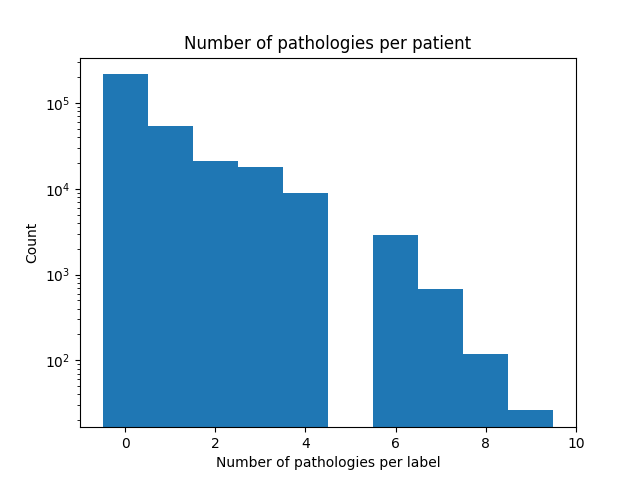
\includegraphics[width=\textwidth]{plots/disease_count_log}
     \caption{Histogram of classes per image for the CIUSSS training dataset}
     \label{fig:classes_per_image}

\end{figure}

    Now come the tricky part where we get in the wood inside of getting out. While the data processing described earlier
    is accurate, it is also general and do not reflect the specificty of our data! Two main problem arise.

    Firstly, as mentionned earlier, the data is unbalanced! While typically , we would simply undersample the over-represented
    categories or the opposite, oversample the under-represented classes, it is not an option here. Looking closely at the data \ref{fig:classes_per_image},
    we can see our problem is not a simple classification, but a multilabel classification tasks where more than one class might be present
    in the input! We also see that we have a lot of images with no pathology at all. This is a problem as it means that the model will be biased toward answering no pathology are present. We therefore need to undersample this category!



    To resolve this , we can try some version of undersampling to partially mitigate the imbalance, but a better solution exists. We can assign each positive example
    of a class with a weight, therefore increasing the importance of the positive examples of the under-represented classes. This is
    done by using the class weights parameter of the loss function. This is a good solution, but it is not perfect of course as one class might have a higher preponderance in the loss
    function.

    To mitigate this, we could use a weighted loss function, which will weight the loss of each class according to the class weights. This could be interesting as a future improvement.


    Secondly, our data does not come in the form of a simple image. The input is composed of multiple images present in the patient file for a specific exam, typically between 1 and 4 images. While a RNN could be use to deal
    with a sequence of image, no such model exist for medical imaging. Instead, we will use a CNN to process each image independently, and combine the output with a simple addition before applying the sigmoid activation function.

    To further simplify the model, we also explored two other option

    \subsection{Option 1 : Only use 1 frontal image}
        Our first attempt was to use only one frontal image per patient. This is a simple solution, but it is not optimal as it does not take into account the other images present in the patient file.
        However, we quickly realize that this was not a good idea as the model was underperforming with some specific pathologies. This was most
        likely due to these pathologies having been identified through the other images present in the patient file, and especially the lateral images.
        Further investigation confirmed our hypothesis, as some pathologies like pleural effusion were mostly confirmed by the lateral images.

    \subsection{Option 2 : Use two different set of weights for the feature extraction of frontal vs lateral images}

        To ensure the model learned in an optimal manner from both lateral and frontal images, we tried to use two different set of weights for the feature extraction of frontal vs lateral images. This however
        effectively double the number of parameters to train, and led to a significant increase in the model capacity and overfitting. This option was therefore also rejected.

        % link to document?
    Finally , we opted to use two of the images present in the patient file, and to combine the output of the CNN with a simple addition before applying the sigmoid activation function. This is a simple solution, but it is not optimal as it does not take into account the other images present in the patient file.
    It however will help simplify training as the model will almost always have the same number of input images (2, more rarely 1), and will also help with the generalization of the model as it will be trained on a wider variety of images.

    To undersample the empty images, we will ponder them with a weight of 0.1, and the other images with a weight of 1. This will effectively leave us with a dataset containing the equivalent of only about 20 000 empty images.





    \section{Model architecture}

    \subsection{Model 1 : DenseNet \cite{densenet}}


    \begin{figure}[h]

         \centering
         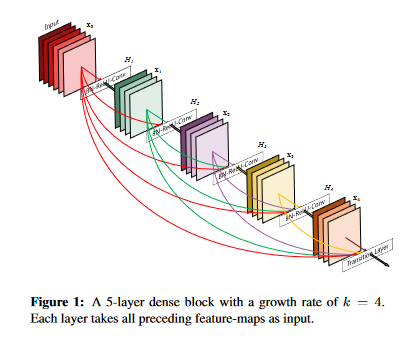
\includegraphics[width=0.5 \textwidth]{plots/densenet_figure}
         \caption{Figure 1 from the densenet paper \cite{densenet}. It shows how the layers are all interconnected}
         \label{fig:densenet_figure}

    \end{figure}

        The densenet model is a CNN model that is composed of dense blocks. Each dense block is composed of a series of convolutional layers,
        each of which is connected to all the previous layers in the block (see \ref{fig:densenet_figure}). This allows the model to learn features at different scales, and to
        combine them in a more efficient manner. The model is also composed of a transition layer, which is used to reduce the number of feature maps
        and to control the growth of the model. The model is also composed of a classifier, which is composed of a global average pooling layer and a fully connected layer.



        This model released in 2018 improved on ResNet with its dense blocks, and was the state of the art for a while. The stanford team working on ChexNet found it was the best model available to achieve the highest AUC on CXR images \cite{chexnet}.


    \subsection{Model 2 : ConvNeXt \cite{convnext}}


\begin{figure}[h]

     \centering
     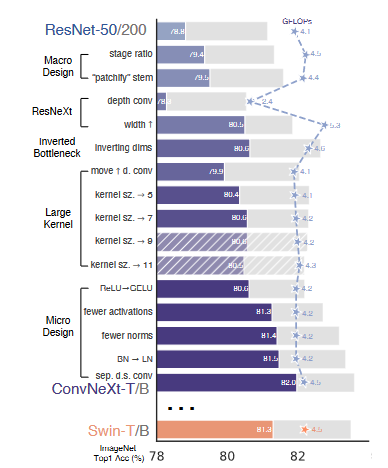
\includegraphics[width=0.5 \textwidth]{plots/convnext_graph}
     \caption{Figure 2 from the ConvNeXt paper \cite{convnext}. It details the different improvement made to the
     resnet architecture and the gain in performance obtained following each modification.}
     \label{fig:convnext}

\end{figure}

        The ConvNeXt model is another CNN model, this time released in 2020 and improving on the default Resnet architecture once again.
        They gradually implemented many of the features of vision transformers in order to "modernize" the typical CNN architecture. In doing sp,
        they created an architecture which outperformed many SOTA models on the ImageNet competititon.

        The details of these modifications can be seen in the figure \ref{fig:convnext}, which is taken from their paper.
        It replaced densenet as the "default" convolutionnal model


    \subsection{Model 3 : EfficientNet \cite{efficientnet}}

        T

    \subsection{Model 4 : Deit \& Transformers \cite{deit} \cite{image16x16}}



    \section{Training}

    \section{Preliminary Results}





    \section{Analysis of the results}



    \newpage
    % REFERENCES
    {
    \small
    \printbibliography
    }
\end{document}